\documentclass[11pt,a4paper]{book}
\usepackage{lmodern}
\usepackage{amssymb,amsmath}
\usepackage{ifxetex,ifluatex}
\usepackage{fixltx2e} % provides \textsubscript
\ifnum 0\ifxetex 1\fi\ifluatex 1\fi=0 % if pdftex
  \usepackage[T1]{fontenc}
  \usepackage[utf8]{inputenc}
\else % if luatex or xelatex
  \ifxetex
    \usepackage{mathspec}
  \else
    \usepackage{fontspec}
  \fi
  \defaultfontfeatures{Ligatures=TeX,Scale=MatchLowercase}
\fi
% use upquote if available, for straight quotes in verbatim environments
\IfFileExists{upquote.sty}{\usepackage{upquote}}{}
% use microtype if available
\IfFileExists{microtype.sty}{%
\usepackage{microtype}
\UseMicrotypeSet[protrusion]{basicmath} % disable protrusion for tt fonts
}{}
\usepackage{hyperref}
\PassOptionsToPackage{usenames,dvipsnames}{color} % color is loaded by hyperref
\hypersetup{unicode=true,
            pdftitle={Relativistic Cosmology Part 2},
            pdfauthor={Dr Vicky Scowcroft},
            colorlinks=true,
            linkcolor=black,
            citecolor=magenta,
            urlcolor=magenta,
            breaklinks=true}
\urlstyle{same}  % don't use monospace font for urls
\usepackage{natbib}
\bibliographystyle{apalike}
\usepackage{longtable,booktabs}
\usepackage{graphicx}
% grffile has become a legacy package: https://ctan.org/pkg/grffile
\IfFileExists{grffile.sty}{%
\usepackage{grffile}
}{}
\makeatletter
\def\maxwidth{\ifdim\Gin@nat@width>\linewidth\linewidth\else\Gin@nat@width\fi}
\def\maxheight{\ifdim\Gin@nat@height>\textheight\textheight\else\Gin@nat@height\fi}
\makeatother
% Scale images if necessary, so that they will not overflow the page
% margins by default, and it is still possible to overwrite the defaults
% using explicit options in \includegraphics[width, height, ...]{}
\setkeys{Gin}{width=\maxwidth,height=\maxheight,keepaspectratio}
\IfFileExists{parskip.sty}{%
\usepackage{parskip}
}{% else
\setlength{\parindent}{0pt}
\setlength{\parskip}{6pt plus 2pt minus 1pt}
}
\setlength{\emergencystretch}{3em}  % prevent overfull lines
\providecommand{\tightlist}{%
  \setlength{\itemsep}{0pt}\setlength{\parskip}{0pt}}
\setcounter{secnumdepth}{5}

%%% Use protect on footnotes to avoid problems with footnotes in titles
\let\rmarkdownfootnote\footnote%
\def\footnote{\protect\rmarkdownfootnote}

%%% Change title format to be more compact
\usepackage{titling}

% Create subtitle command for use in maketitle
\providecommand{\subtitle}[1]{
  \posttitle{
    \begin{center}\large#1\end{center}
    }
}

\setlength{\droptitle}{-2em}

  \title{Relativistic Cosmology Part 2}
    \pretitle{\vspace{\droptitle}\centering\huge}
  \posttitle{\par}
    \author{Dr Vicky Scowcroft}
    \preauthor{\centering\large\emph}
  \postauthor{\par}
      \predate{\centering\large\emph}
  \postdate{\par}
    \date{Semester 2, 2019/20}

\usepackage{booktabs}
\usepackage{amsthm}
\usepackage{titlesec}
\newcommand{\sectionbreak}{\clearpage}

\makeatletter
\def\thm@space@setup{%
  \thm@preskip=8pt plus 2pt minus 4pt
  \thm@postskip=\thm@preskip
}
\makeatother

\renewcommand*\familydefault{\sfdefault} %% Only if the base font of the document is to be sans serif
%\usepackage[includefoot, , top=20mm, left=20mm, right=50mm, bottom=15mm, footskip=15mm]{geometry}
\usepackage{fancyhdr}

\pagestyle{fancy}

\fancyhead{}

\renewcommand{\footrulewidth}{0.4pt}
\setcounter{secnumdepth}{2}


%\renewcommand{\chaptername}{Section}

\parskip=0.5cm
\parindent 10pt

\newcommand{\ps}[0]{4mm}
\renewcommand{\theequation}{\arabic{section}.\arabic{equation}}

%\usepackage[fontsize=11]{scrextend}

\begin{document}
\maketitle

{
\hypersetup{linkcolor=black}
\setcounter{tocdepth}{1}
\tableofcontents
}
\hypertarget{unit-overview}{%
\chapter*{Unit Overview}\label{unit-overview}}
\addcontentsline{toc}{chapter}{Unit Overview}

The aim of this section of PH40112 is to present the observations and
theory underpinning modern Cosmology. It is complementary to the first
half of PH40112, which focusses on General Relativity and its
applications to Cosmology. At the end of this course, you should be
able to describe the key ideas of Cosmology, comparing and contrasting
different observational techniques and Cosmological models. You should
understand the implications for the fate of the Universe arising from
these different models, and discuss the open questions being addressed
by current state of the art experiments. You should also be able to
assess how systematic errors and experimental uncertainties affect
cosmological experiments, in particular how these affect our ability
to discriminate between different models of the Universe's evolution.

\hypertarget{topics-and-schedule}{%
\section*{Topics and Schedule}\label{topics-and-schedule}}
\addcontentsline{toc}{section}{Topics and Schedule}

The planned schedule for sessions is as follows:

\begin{longtable}[]{@{}llcr@{}}
\toprule
\begin{minipage}[b]{0.05\columnwidth}\raggedright
Week\strut
\end{minipage} & \begin{minipage}[b]{0.09\columnwidth}\raggedright
Date\strut
\end{minipage} & \begin{minipage}[b]{0.19\columnwidth}\centering
Session\strut
\end{minipage} & \begin{minipage}[b]{0.55\columnwidth}\raggedleft
Topic\strut
\end{minipage}\tabularnewline
\midrule
\endhead
\begin{minipage}[t]{0.05\columnwidth}\raggedright
7\strut
\end{minipage} & \begin{minipage}[t]{0.09\columnwidth}\raggedright
16/3\strut
\end{minipage} & \begin{minipage}[t]{0.19\columnwidth}\centering
Lecture 1\strut
\end{minipage} & \begin{minipage}[t]{0.55\columnwidth}\raggedleft
Introduction to Observational Cosmology\strut
\end{minipage}\tabularnewline
\begin{minipage}[t]{0.05\columnwidth}\raggedright
\strut
\end{minipage} & \begin{minipage}[t]{0.09\columnwidth}\raggedright
19/3\strut
\end{minipage} & \begin{minipage}[t]{0.19\columnwidth}\centering
Lecture 2\strut
\end{minipage} & \begin{minipage}[t]{0.55\columnwidth}\raggedleft
Equations of the Expanding Universe\strut
\end{minipage}\tabularnewline
\begin{minipage}[t]{0.05\columnwidth}\raggedright
\strut
\end{minipage} & \begin{minipage}[t]{0.09\columnwidth}\raggedright
20/3\strut
\end{minipage} & \begin{minipage}[t]{0.19\columnwidth}\centering
Lecture 3\strut
\end{minipage} & \begin{minipage}[t]{0.55\columnwidth}\raggedleft
Composition of the Universe\strut
\end{minipage}\tabularnewline
\begin{minipage}[t]{0.05\columnwidth}\raggedright
8\strut
\end{minipage} & \begin{minipage}[t]{0.09\columnwidth}\raggedright
23/3\strut
\end{minipage} & \begin{minipage}[t]{0.19\columnwidth}\centering
Lecture 4\strut
\end{minipage} & \begin{minipage}[t]{0.55\columnwidth}\raggedleft
Observational Parameters\strut
\end{minipage}\tabularnewline
\begin{minipage}[t]{0.05\columnwidth}\raggedright
\strut
\end{minipage} & \begin{minipage}[t]{0.09\columnwidth}\raggedright
26/3\strut
\end{minipage} & \begin{minipage}[t]{0.19\columnwidth}\centering
Lecture 5\strut
\end{minipage} & \begin{minipage}[t]{0.55\columnwidth}\raggedleft
Observational Techniques\strut
\end{minipage}\tabularnewline
\begin{minipage}[t]{0.05\columnwidth}\raggedright
\strut
\end{minipage} & \begin{minipage}[t]{0.09\columnwidth}\raggedright
27/3\strut
\end{minipage} & \begin{minipage}[t]{0.19\columnwidth}\centering
Lecture 6\strut
\end{minipage} & \begin{minipage}[t]{0.55\columnwidth}\raggedleft
The \(\Lambda\)CDM Model\strut
\end{minipage}\tabularnewline
\begin{minipage}[t]{0.05\columnwidth}\raggedright
9\strut
\end{minipage} & \begin{minipage}[t]{0.09\columnwidth}\raggedright
30/3\strut
\end{minipage} & \begin{minipage}[t]{0.19\columnwidth}\centering
Lecture 7\strut
\end{minipage} & \begin{minipage}[t]{0.55\columnwidth}\raggedleft
Dark Matter\strut
\end{minipage}\tabularnewline
\begin{minipage}[t]{0.05\columnwidth}\raggedright
\strut
\end{minipage} & \begin{minipage}[t]{0.09\columnwidth}\raggedright
2/4\strut
\end{minipage} & \begin{minipage}[t]{0.19\columnwidth}\centering
\textbf{Discussion session}\strut
\end{minipage} & \begin{minipage}[t]{0.55\columnwidth}\raggedleft
Current Research Topics\strut
\end{minipage}\tabularnewline
\begin{minipage}[t]{0.05\columnwidth}\raggedright
\strut
\end{minipage} & \begin{minipage}[t]{0.09\columnwidth}\raggedright
3/4\strut
\end{minipage} & \begin{minipage}[t]{0.19\columnwidth}\centering
Lecture 8\strut
\end{minipage} & \begin{minipage}[t]{0.55\columnwidth}\raggedleft
Structures in the Universe\strut
\end{minipage}\tabularnewline
\begin{minipage}[t]{0.05\columnwidth}\raggedright
10\strut
\end{minipage} & \begin{minipage}[t]{0.09\columnwidth}\raggedright
20/4\strut
\end{minipage} & \begin{minipage}[t]{0.19\columnwidth}\centering
Lecture 9\strut
\end{minipage} & \begin{minipage}[t]{0.55\columnwidth}\raggedleft
Inflation\strut
\end{minipage}\tabularnewline
\begin{minipage}[t]{0.05\columnwidth}\raggedright
\strut
\end{minipage} & \begin{minipage}[t]{0.09\columnwidth}\raggedright
23/4\strut
\end{minipage} & \begin{minipage}[t]{0.19\columnwidth}\centering
Lecture 10\strut
\end{minipage} & \begin{minipage}[t]{0.55\columnwidth}\raggedleft
The Evolving Universe\strut
\end{minipage}\tabularnewline
\begin{minipage}[t]{0.05\columnwidth}\raggedright
\strut
\end{minipage} & \begin{minipage}[t]{0.09\columnwidth}\raggedright
24/4\strut
\end{minipage} & \begin{minipage}[t]{0.19\columnwidth}\centering
Problems Class\strut
\end{minipage} & \begin{minipage}[t]{0.55\columnwidth}\raggedleft
Problems Class\strut
\end{minipage}\tabularnewline
\begin{minipage}[t]{0.05\columnwidth}\raggedright
11\strut
\end{minipage} & \begin{minipage}[t]{0.09\columnwidth}\raggedright
27/4\strut
\end{minipage} & \begin{minipage}[t]{0.19\columnwidth}\centering
Problems Class\strut
\end{minipage} & \begin{minipage}[t]{0.55\columnwidth}\raggedleft
Problems Class\strut
\end{minipage}\tabularnewline
\begin{minipage}[t]{0.05\columnwidth}\raggedright
\strut
\end{minipage} & \begin{minipage}[t]{0.09\columnwidth}\raggedright
30/4\strut
\end{minipage} & \begin{minipage}[t]{0.19\columnwidth}\centering
Problems Class\strut
\end{minipage} & \begin{minipage}[t]{0.55\columnwidth}\raggedleft
Problems Class\strut
\end{minipage}\tabularnewline
\begin{minipage}[t]{0.05\columnwidth}\raggedright
\strut
\end{minipage} & \begin{minipage}[t]{0.09\columnwidth}\raggedright
1/5\strut
\end{minipage} & \begin{minipage}[t]{0.19\columnwidth}\centering
Revision Session\strut
\end{minipage} & \begin{minipage}[t]{0.55\columnwidth}\raggedleft
Revision Session and Q\&A\strut
\end{minipage}\tabularnewline
\begin{minipage}[t]{0.05\columnwidth}\raggedright
12\strut
\end{minipage} & \begin{minipage}[t]{0.09\columnwidth}\raggedright
4/5 - 7/5\strut
\end{minipage} & \begin{minipage}[t]{0.19\columnwidth}\centering
Office hours\strut
\end{minipage} & \begin{minipage}[t]{0.55\columnwidth}\raggedleft
Revision week. Office hours will be posted closer to the date.\strut
\end{minipage}\tabularnewline
\bottomrule
\end{longtable}

Lectures have been front-loaded for this section of the course. Problem sheets will be released once the relavent material has been covered, but formal problems classes will not take place until weeks 10 and 11.

The schedule was last updated on 13th March. Changes to the planned schedule will be posted here and on the moodle page.

\hypertarget{discussion-session---thursday-2ndapril}{%
\section*{Discussion session - Thursday 2ndApril}\label{discussion-session---thursday-2ndapril}}
\addcontentsline{toc}{section}{Discussion session - Thursday 2ndApril}

The session on Thursday April 2nd will be a discussion session, covering three journal publications using different techniques used to estimate cosmological parameters. You will each be assigned to a group during week 8 and the group assignments and corresponding papers will be posted to Moodle. After the session, summaries of the discussions will be uploaded to Moodle and the relavent section of these notes.

If the date and/or format of this session needs to change, updates will be posted here and on the Moodle forum.

\hypertarget{suggested-textbook}{%
\section*{Suggested textbook}\label{suggested-textbook}}
\addcontentsline{toc}{section}{Suggested textbook}

This section of the course closely follows several chapters of \emph{An
Introduction to Modern Cosmology: 3rd edition} by Liddle.
You may find it helpful to refer to this book or others such as \emph{The
Oxford companion to Cosmology} by Liddle and Loveday, which is
available in the University library.

\hypertarget{lecture-notes-slides-recordings}{%
\section*{Lecture notes, slides, recordings}\label{lecture-notes-slides-recordings}}
\addcontentsline{toc}{section}{Lecture notes, slides, recordings}

Written notes for lectures 1 - 10 will be made available online in html and PDF format. The html notes are available at \url{https://vickyscowcroft.github.io/PH40112_rmd/} and will be updated throughout the course. PDF versions of the notes will be posted to the course Moodle page. The html notes have been designed so that the maths content is compatible with screen readers.

Lectures will follow the same general structure as the written notes, but will not be identical - i.e.~they will not be `skeleton' notes for you to fill in the blanks. They are designed to support your learning of the lecture material, so you may find it useful to make your own notes during the session.

PDF versions of the slides for each session will be posted on Moodle before each session. If you need these in an alternative format please let me know.

All sessions will be recorded with Panopto and can be accessed in the usual way.

\hypertarget{ch:intro_obs}{%
\chapter{Overview of Observational Cosmology}\label{ch:intro_obs}}

This section introduces the observational foundation of Cosmology. It
builds upon the material in PH30111: Introduction to Galaxies and
Cosmology. Some material may be familiar to you, but the origins and
derivations of the equations will be discussed in more depth, and will
include the relativistic treatment introduced in the first half of this
course.

\hypertarget{sec:cosmoprinciple}{%
\section{The Cosmological Principle}\label{sec:cosmoprinciple}}

The Cosmological Principle is the belief that \textbf{our position in the
Universe is not special in any way}.

If the Cosmological Principle holds, then there is no special position
in the Universe, meaning that it should be the same everywhere (i.e.~it
should be \textbf{homogeneous}), and it should have no preferred direction
(i.e.~it should be \textbf{isotropic})

Clearly the Universe is not isotropic and homogeneous on small scales --
the distributions of things like stars, planets and galaxies give more
or less dense regions locally. But on a large scale, the Universe does
display homogeneity and isotropy; Galaxy clusters are spread over the
Universe and not concentrated to one side, and the CMB has only very
tiny fluctuations.

\hypertarget{sec:history}{%
\section{A brief history of the Universe}\label{sec:history}}

The `Cosmic Calendar' shown in
Figure \ref{fig:cosmic-calendar} condenses the evolution of the Universe
to a timescale of 1 calendar year. If the Big Bang occurred on January
1st, human life wouldn't exist until 11:52pm on 31st December! The
formation of the Solar System would have occurred in September, and our
home in the Galaxy, the disk of the Milky Way, would have formed in May.

As
Figure \ref{fig:cosmic-calendar} shows, our understanding of how the
Universe and our place in it has evolved over time uses different
sources of evidence depending on the time frame. Our knowledge of recent
history comes from written records, while our knowledge of the formation
of the Solar System and the evolution of Earth comes from geology.
However, to understand how the Universe as a whole came to be, we must
look further back in time.

\textbackslash{}begin\{figure\}
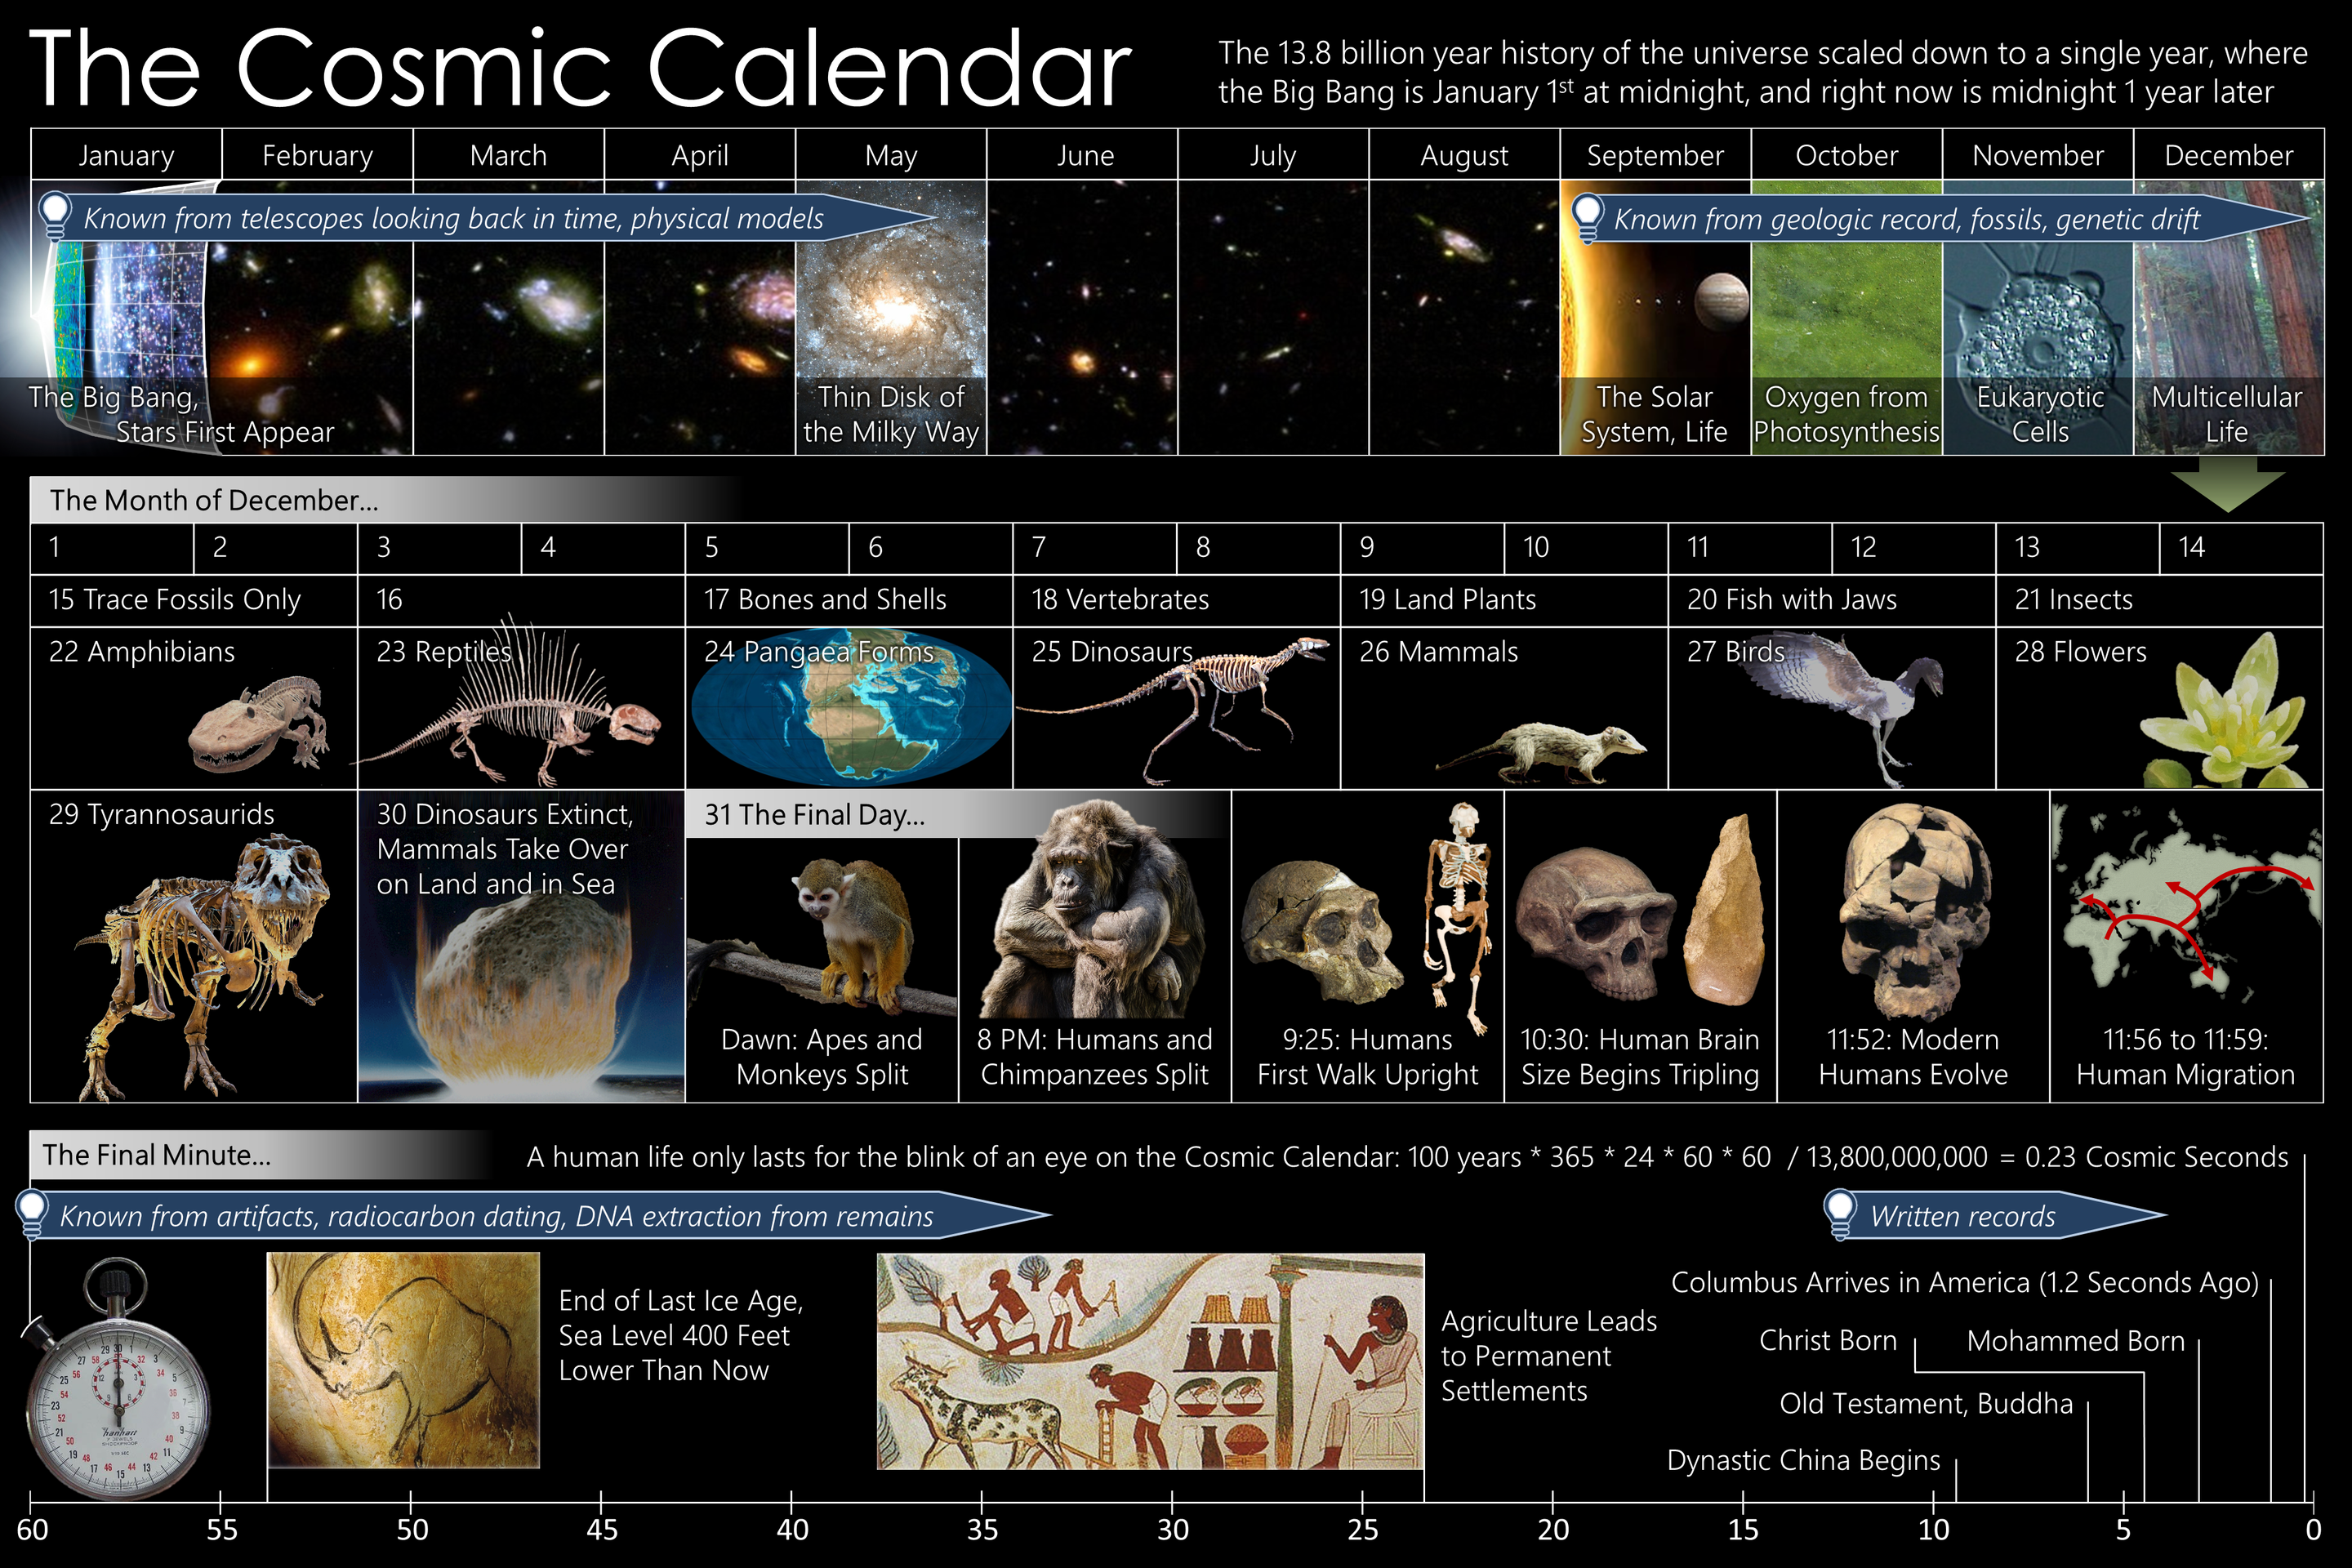
\includegraphics[width=1\linewidth]{Images/CosmicCalendar} \textbackslash{}caption\{The Cosmic Calendar. Credit: By Efbrazil, CC BY-SA 3.0 \citep{wikipedia_2020}.\}\label{fig:cosmic-calendar}
\textbackslash{}end\{figure\}

Figure \ref{fig:evo-universe} illustrates our current understanding of
the evolution of the Universe, starting with the Big Bang, through to
the Universe as we see it today. This section gives a brief history of
the evolution; topics will be covered in further detail later in the
course. We will not move through these chronologically in this course;
instead this is intended to give you an overview of how the different
ideas we cover come together.

\begin{figure}
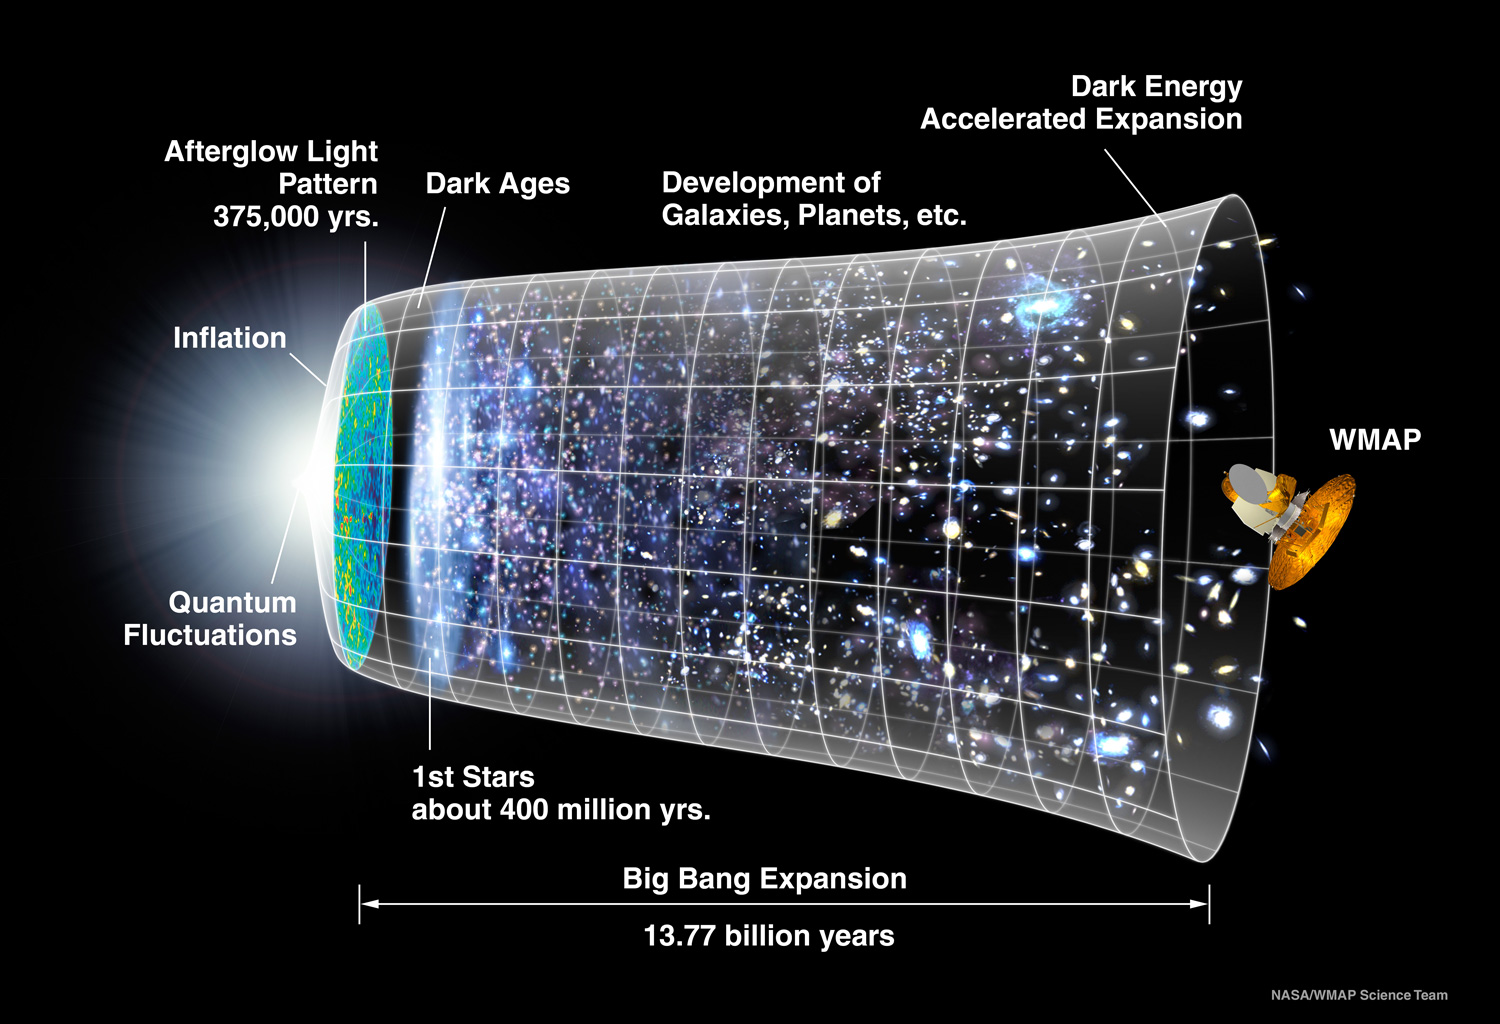
\includegraphics[width=1\linewidth]{Images/060915_CMB_Timeline150_annotated} \caption{Evolution of the Universe. Original image credit: NASA/WMAP Science Team}\label{fig:evo-universe}
\end{figure}

\hypertarget{sec:first_second}{%
\section{The first second}\label{sec:first_second}}

The first second after the Big Bang was quite dramatic. Highlights of
this time are given below. Bear in mind that all of the following
happens in less time than it takes for your heart to beat twice.

\begin{itemize}
\tightlist
\item
  The Big Bang \((t = 0)\)
\end{itemize}

The Universe began with the Big Bang, rapidly expanding from an initial
singularity.

\begin{itemize}
\tightlist
\item
  Planck epoch \((t = 10^{-43}~s)\)
\end{itemize}

The Planck epoch refers to the stage when the Universe's density
exceeded a critical density, such that the energy scale is greater than
the Planck scale. At this scale, quantum effects are important even for
gravitational physics.

\begin{itemize}
\tightlist
\item
  Separation of forces \((10^{-43}~s < t < 10^{-36}~s)\)
\end{itemize}

After the Planck epoch, other fundamental forces start to separate out.
First, the gravitational force and electronuclear force decouple, then
the electronuclear force separates out into the strong and electroweak
forces.

\begin{itemize}
\tightlist
\item
  Inflation \((t < 10^{-32}~s)\)
\end{itemize}

Early in its evolution, the Universe underwent a period of rapid
inflation, expanding by a factor of \(10^{78}\) (or \(10^{26}\) in each of
the three spatial dimensions). Under this rapid expansion, an area of
space of the order of 1~nm\(^{3}\) would expand to approximately
30~pc\(^{3}\) (equivalent to around 100~lyr\(^{3})\). Such expansion must
occur at greater than the speed of light (\(c\)). However, as it is the
metric of space time that is expanding, the limitation of exceeding \(c\)
is not applicable, and inflation can occur.

\begin{itemize}
\tightlist
\item
  Electroweak symmetry breaking \((t = 10^{-12}~s)\)
\end{itemize}

After inflation, the electroweak force separates into the
electromagnetic and weak nuclear forces.

\begin{itemize}
\tightlist
\item
  Quark epoch \((t = 10^{-12}~s)\)
\end{itemize}

At the same time as electroweak symmetry breaking, the energy density of
the Universe has decreased such that matter can exist in the form of
quarks.

\begin{itemize}
\tightlist
\item
  Baryogenesis \((t = 10^{-11}~s)\)
\end{itemize}

Baryogenesis is the stage where matter can start to exist in the form of
baryons - e.g.~protons, neutrons. Baryogensis should have produced both
baryons and anti-baryons (e.g.~protons and anti-protons). Current
evidence - i.e.~the fact that we exist and are composed of baryons -
shows that there must have been an asymmetry in the proportions of
baryons/anti-baryons, otherwise they would have all have annihilated.
The Baryogenesis process and baryon asymmetry are current areas of
research.

\begin{itemize}
\tightlist
\item
  Hadron epoch \((10^{-6}~s < t < 1~s)\)
\end{itemize}

The Hadron epoch occurred when the Universe had cooled far enough for
hadrons to exist and dominate the energy density. The proportions of
hadrons and anti-hadrons were similar, such that they were in thermal
equilibrium and mostly annihilated, producing photons, although a small
number of hadrons remained.

\begin{itemize}
\tightlist
\item
  Neutrino decoupling \((t < 1~s)\)
\end{itemize}

Around 1s after the Big Bang, neutrinos decoupled and were free to
propagate through the Universe. Neutrinos have a very small interaction
cross section, so the Cosmic Neutrino Background created at neutrino
decoupling should still exist today. However, as the neutrinos produced
at decoupling have such low energies, it is impossible to detect them
with current experiments.

\begin{itemize}
\tightlist
\item
  Lepton epoch \((1~s < t < 10~s)\)
\end{itemize}

Similar to the Hadron epoch, the Lepton epoch produced both leptons and
anti-leptons (e.g, electrons, muons, neutrinos etc.) These would have
annihilated, producing pairs of photons. A small number of leptons
remain after annihilation.

\hypertarget{sec:after_1s}{%
\section{After the first second:}\label{sec:after_1s}}

The Universe has now been evolving for around 1 s. It has exponentially
expanded, created all the matter and radiation we see (and destroyed a
whole load too), and gone through several rounds of fundamental physical
forces. What else is left to do for the next 13.77 billion years?

\begin{itemize}
\tightlist
\item
  Photon epoch \((10~s < t < 377,000\text{ years})\)
\end{itemize}

After baryons, hadrons and leptons have mostly been annihilated, the
majority of the Universe's energy is dominated by photons.

\begin{itemize}
\tightlist
\item
  Light Element Nucleosynthesis \((2 \text{ mins} < t < 20\text{ mins})\)
\end{itemize}

Nucleosynthesis is the stage where light elements (i.e., Hydrogen,
Deuterium, Helium, Lithium) were formed. Elements heavier than Helium
were very difficult to form due to the large amounts of energy/time
required.

\begin{itemize}
\tightlist
\item
  Matter domination \((t = 47,000\text{ years})\)
\end{itemize}

Around 47,000 years after the Big Bang, the energy density of matter in
the Universe overtakes that of radiation. Matter now becomes the
dominant driver of the Universe's evolution.

\begin{itemize}
\tightlist
\item
  Epoch of recombination and photon decoupling \((t = 377,000\text{ years})\)
\end{itemize}

During the epoch of recombination, ionised particles (e.g.~electrons,
protons) combined to form neutral atoms. At this stage, the matter
density was such that photons only had a short path length before they
would interact with an ionised particle, making the Universe opaque. As
recombination progressed, and ionised particles combined into neutral
atoms, the photon path length increased, making the Universe transparent
to photons. The decoupled photons produced during this time have been
redshifted by the expansion of the Universe, so we now observe them as
the Cosmic Microwave Background (CMB).

\begin{itemize}
\tightlist
\item
  Dark Ages \((380,000 \text{ years}< t < 1\text{ Gyr})\)
\end{itemize}

At this time, photons were free to stream through the Universe. However,
light-producing systems such as stars had not yet formed, so the
Universe was "dark". The only sources of photons were those from the
CMB, and those emitted from neutral Hydrogen atoms at 21~cm.

\begin{itemize}
\tightlist
\item
  Formation of structure \((150\text{ Myr} < t < 1\text{ Gyr})\)
\end{itemize}

Structure forms hierarchically in the Universe; smaller structures form
first and are built up into larger ones. The first structures to form in
the Universe were stars, dwarf galaxies, and quasars. The first
population of stars (Population III stars) are thought to have formed
around t~\(=700\)~Myr. Pop III stars are yet to be detected
observationally.

\begin{itemize}
\tightlist
\item
  Epoch of reionisation \((250 \text{ Myr} < t 1\text{ Gyr})\)
\end{itemize}

Pop III stars introduced a new source of radiation into the Universe.
During the epoch of reionisation this radiation ionised the neutral
Hydrogen, creating a plasma of protons and electrons. The epoch of
reionisation most likely lasted until around 1~Gyr, when the Population
III stars died off. At this time, the ionised Hydrogen gradually
recombined to neutral Hydrogen once more.

\begin{itemize}
\tightlist
\item
  Formation of Galaxies and Clusters \((t\)\textgreater{}\(1 \text{ Gyr})\)
\end{itemize}

"Large" galaxies and galaxy clusters formed from around t = 1 Gyr.
These would have first comprised Population II stars, which, unlike Pop
III stars, we do observe today. Later, the next generation of stars, Pop
I, formed.

\begin{itemize}
\tightlist
\item
  Dark Energy epoch \((t > 9.8 \text{ Gyr})\)
\end{itemize}

We are currently believed to be in the dark energy epoch, where the
energy density of the Universe is dominated by the dark energy
contribution. While we don't know the nature of dark energy, its effects
are seen as driving the expansion of the Universe so it is not just
getting larger, but the expansion itself is accelerating.

\hypertarget{sec:expanding_intro}{%
\section{The Expanding Universe}\label{sec:expanding_intro}}

The first observational evidence that the Universe is expanding was
found by Edwin Hubble \citep{1929Hubble}. By measuring the distances
to nearby galaxies using the Cepheid Leavitt Law, and comparing
these distances to the galaxies' redshifts. Hubble measured the
expansion rate of the Universe (the \textbf{Hubble constant, \(\mathbf{H_0}\)})
to be approximately 500 km s\(^{-1}\) Mpc\(^{-1}\). Hubble's observations
are shown in
Figure \ref{fig:hubble-h0-diagram}. Throughout this course we will
explore how observations of the Universe have developed over the past
century, increasing in precision and accuracy, leading to our current
understanding of Cosmology.

\begin{figure}
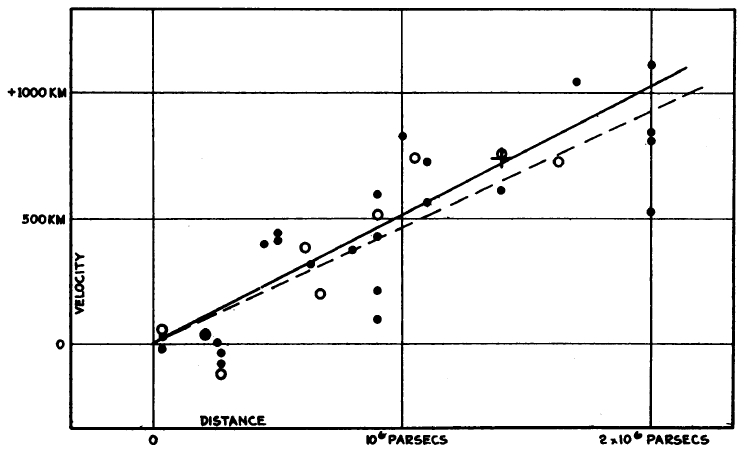
\includegraphics[width=1\linewidth]{Images/hubble-diagram} \caption{The first observational evidence of the expanding Universe. His first measurement of the expansion rate, now known as the Hubble constant, was 500 km s$^{-1}$ Mpc$^{-1}$. From [@1929Hubble].}\label{fig:hubble-h0-diagram}
\end{figure}

\hypertarget{ch:eqs_of_expanding}{%
\chapter{Equations of the Expanding Universe}\label{ch:eqs_of_expanding}}

\hypertarget{sec:metric}{%
\section{Metric of space-time}\label{sec:metric}}

Consider a flat piece of paper where points can be specified by
coordinates \(x_1\) and \(x_2\). The distance between two points is given by
\begin{equation}
\Delta s^2 = \Delta x_{1}^{2} + \Delta x_{2}^{2}
\label{eq:dist01}
\end{equation}
where
\(\Delta x_{1}^{2}\) and \(\Delta x_{2}^{2}\) are the separations in the
\(x_1\) and \(x_2\) coordinates.

What about if we replaced the paper with a rubber sheet that can expand?
The coordinate system \(x_1\)--\(x_2\) will expand with the sheet, and the
physical distance between the points will change over time.

Assuming that the expansion is uniform over the whole sheet, we now have
\begin{equation}
\Delta s^2 = a^2(t)\left[\Delta x_{1}^{2} + \Delta x_{2}^{2}\right]
\label{eq:comoving01}
\end{equation}
where \(a(t)\) measures the rate of expansion. \(x_1\) and \(x_2\) are
\textbf{comoving coordinates}.

Our current definition of \(\Delta s\) only depends on the spatial
distance between the points. However, in general relativity, we have to
consider 4-dimensional space time, which may be curved.

In this case, the distance becomes
\begin{equation}
ds^2 = \sum_{\mu, \nu} g_{\mu\nu} dx^{\mu} dx^{\nu}
\label{eq:ds-gr-metric}
\end{equation}
where \(g_{\mu\nu}\) is the metric and \(\mu\) and \(\nu\) are indices taking
the values 0, 1, 2, 3. \(x^{0}\) is the time coordinate and
\(x^{1}, x^{2}, x^{3}\) are the spatial coordinates.

The spatial component of
Equation \eqref{eq:ds-gr-metric} can be simplified by applying the
\textbf{Cosmological Principle} (see Sec. \ref{sec:cosmoprinciple}) - i.e.~the Universe should not have any
preferred locations. This means that \textbf{the spatial component must have
constant curvature at all positions.}

Changing to spherical polar coordinates, we now get
\begin{equation}
ds^2_3 = \dfrac{dr^2}{1 - kr^2} + r^2\left(d\theta^2 + \sin^2\theta d\phi^2\right)
\label{eq:ds-gr-metric-polar}
\end{equation}
where \(ds_3^2\) considers only the spatial dimensions, and \(k\) is a
constant which measures the curvature of space.

Incorporating this into the space-time metric gives
\begin{equation}
ds^2 = -c^2 dt^2 + a^2(t) \left[\dfrac{dr^2}{1 - kr^2} + r^2\left(d\theta^2 + \sin^2\theta d\phi^2\right)\right]
\label{eq:rw-metric}
\end{equation}
Which is the \textbf{Robertson-Walker metric}. Here \(a(t)\) is the \textbf{scale
factor of the Universe} - i.e. \(a(t) = r/r_0,\) where \(r_0\) is \(r\) at
time \(t_0\).

\hypertarget{sec:einstein_eqs}{%
\section{The Einstein Equations}\label{sec:einstein_eqs}}

The Robertson-Walker metric evolves according to Einstein's equation:
\begin{equation}
R_{\mu\nu} - \dfrac{1}{2}g_{\mu\nu}R = \dfrac{8\pi G}{c^4} T_{\mu\nu}
\label{eq:einstein}
\end{equation}

where \({T_{\mu\nu}}\) is the \textbf{energy-momentum tensor} of matter
present, \({R_{\mu\nu}}\) is the \textbf{Ricci tensor}, and \({R}\)
is the \textbf{Ricci scalar}. The Ricci components give the curvature of
space-time.

The energy-momentum tensor is assumed to be symmetric, meaning that
there are potentially 10 Einstein equations. If \(T_{\mu\nu}\) has
additional symmetries, then the number of equations is reduced.

\hypertarget{sec:fluid-eqns}{%
\section{Fluid equation}\label{sec:fluid-eqns}}

We consider that any possible components of the Universe (e.g.~matter,
radiation) can be described as perfect fluids. Perfect fluids have no
viscosity or heat flow, and their equations of state can be described
using only \textbf{density, \(\rho\)} and \textbf{pressure, \(P\)}.

Perfect fluids have a well known relation between energy, \(E\), pressure,
\(P\), and temperature, \(T\):
\begin{equation}
dE + PdV = TdS
\label{eq:de}
\end{equation}
where \(dV\) is the change in volume, and \(dS\) is the
change in entropy.

If we consider a sphere of radius \(a\), using
\begin{equation}
E = mc^2
\label{eq:emc2}
\end{equation}
we can relate
the total energy contained within the sphere to its density via
\begin{equation}
E = \dfrac{4\pi}{3}a^3\rho c^2
\label{eq:e-rho}
\end{equation}

Assuming that the sphere is expanding adiabatically, i.e.~there is no
change in entropy (\(dS = 0\)), differentiating
Equation \eqref{eq:de}
with respect to \(t\) gives

\begin{equation}
    \dot{\rho} + 3\dfrac{\dot{a}}{a}\left(\rho + \dfrac{P}{c^2}\right) = 0
\label{eq:fluid}
\end{equation}
where \(\dot{x} = \dfrac{dx}{dt}, \ddot{x} = \dfrac{d^2x}{dt^2}\), etc. Equation \eqref{eq:fluid} is known as the \textbf{fluid equation}.

As the energy of the perfect fluid depends only on \(P\) and \(\rho\), the
energy-momentum tensor for a perfect fluid is therefore
\begin{equation}
T_{\mu\nu} = \text{diag}\left(-\rho c^2, P, P, P\right)
\label{eq:per-fluid}
\end{equation}
This results
in two independent Einstein equations, the time-time solution and the
space-space solution.

\hypertarget{sec:ricci}{%
\section{Ricci tensor and Ricci scalar}\label{sec:ricci}}

Deriving the full Ricci tensor is beyond the scope of this course. The
following is provided for completeness. The components of the Ricci
tensor that are not equal to zero are those where \(\mu = \nu\), such that

\begin{itemize}
\item
  \(R_{tt} = -3\dfrac{\ddot{a}}{a}\)
\item
  \(R_{rr} = \dfrac{a\ddot{a}}{1 - kr^2} + \dfrac{2\dot{a}^2}{1 - kr^2} + \dfrac{2k}{1-kr^2}\)
\item
  \(R_{\theta\theta} = r^2a\ddot{a} + 2r^2\dot{a}^2 + 2kr^2\)
\item
  \(R_{\phi\phi} = r^2 a\ddot{a}\sin^2\theta + 2r^2\dot{a}^2\sin^2\theta + 2kr^2 \sin^2\theta\)
\end{itemize}

which simplifies to a diagonal tensor with
\begin{equation}
R_{tt}= -3\dfrac{\ddot{a}}{a}
\label{eq:ric-tt}
\end{equation}
and
\begin{equation}
R_{ii} = \dfrac{-g_{ii}}{a^2}\left(a\ddot{a} + 2\dot{a}^2 + 2k\right)
\label{eq:ric-ii}
\end{equation}

The Ricci scalar becomes
\begin{equation}
R = g_{ik}R_{ik} = - 6\dfrac{\ddot{a}}{a} - 6\left(\dfrac{\dot{a}}{a}\right)^2 - 6\dfrac{k}{a^2}
\label{eq:ric-scal}
\end{equation}

\hypertarget{sec:friedman}{%
\section{Friedman Equation}\label{sec:friedman}}

Using the time-time solution of the Einstein equation gives
\begin{equation}
    \left(\dfrac{\dot{a}}{a}\right)^2 + \dfrac{kc^2}{a^2} = \dfrac{8\pi G}{3}\rho
\label{eq:friedman}
\end{equation}
which is the \textbf{Friedman equation}.

The space-space solution follows in a similar way:

\begin{equation}
2\dfrac{\ddot{a}}{a} + \left(\dfrac{\dot{a}}{a}\right)^2 + \dfrac{kc^2}{a^2} = -8\pi G \dfrac{P}{c^2}
\label{eq:acc-part}
\end{equation}

Which looks odd right now, but by subtracting the Friedman equation (Eqn. \eqref{eq:friedman}) we find:
\begin{equation}
    \dfrac{\ddot{a}}{a} = -\dfrac{4\pi G}{3}\left(\rho + \dfrac{3P}{c^2}\right)
\label{eq:acceleration}
\end{equation}

which is the known as the \textbf{acceleration equation}.

\hypertarget{sec:natural_units}{%
\section{\texorpdfstring{Natural units a.k.a. where have all the \(c^2\)'s gone?}{Natural units a.k.a. where have all the c\^{}2's gone?}}\label{sec:natural_units}}

From this point forward, you will see that the factor
\(\left(k c^2/a^2\right)\) in the Friedman equation will magically become
\(\left(k/a^2\right)\). This is because we often like to use \textbf{natural
units} in Cosmology. Mass density \(\left(\rho\right)\) and energy
density \(\left(\epsilon\right)\) are often used interchangeably in
Cosmology, and are related by \(\epsilon = \rho c^2\). By converting to
natural units, i.e.~setting \(c=1\), mass density and energy density are
equivalent. As you will see later, many important cosmological
parameters are expressed in dimensionless units (e.g.~the density
parameters, discussed in sections XXXX. So don't worry about our missing \(c^2\)
factor, it's just another maths trick.

\hypertarget{sec:alt_friedman}{%
\section{An alternative derivation of the Friedman equation}\label{sec:alt_friedman}}

The evolution of the scale factor, \(a\), can be derived using mostly
Newtonian mechanics, in addition to two results from General Relativity:

\begin{itemize}
\item
  \textbf{Birkhoff's theorem} -- for a spherically symmetric system, the
  force due to gravity at radius \(r\) is determined only by the mass
  \emph{interior} to \(r\).
\item
  \textbf{Energy} contributes to the gravitating mass density, such that
  \(E = \rho_m + \dfrac{u}{c^2}\), where \(\rho_m\) is the density of
  matter, and \(u\) is the energy density of radiation and relativistic
  particles.
\end{itemize}

Consider a test particle on the surface of an expanding sphere of radius
\(r\). From \(F= m \ddot{r}\), its equation of motion can be shown to be
\begin{equation}
    \ddot{r} = -\dfrac{4\pi}{3} G \rho r
\label{eq:motion}
\end{equation}

Density is proportional to \(r^{-3}\), so by defining \(r_{0} = 1\), we find
\[\rho = \rho_{0}r^{-3}\] Which can be substituted into Eqn. \eqref{eq:motion} to give:
\begin{equation}
    \ddot{r} = -\dfrac{4\pi}{3}\dfrac{G\rho_0}{r^2}
\label{eq:ddot-r-1}
\end{equation}
If \(\rho_0\) is
non-zero, then \(\ddot{r}\) must also be non-zero. The Universe must
either be expanding or contracting.

To get Eqn.~\eqref{eq:ddot-r-1} into a useful form, we use some clever maths
magic. First, multiply both sides by \(\dot{r}\) to get:
\begin{equation}
\dot{r}\ddot{r} + \dfrac{4\pi}{3}\dfrac{G\rho_{0}}{r^2}\dot{r} = 0
\label{eq:ddot-r-2}
\end{equation}
We can use our mad differentiation skills to recognise that
\begin{equation}
\dfrac{d(\dot{r}^2)}{dt} = 2\dot{r}\ddot{r}
\label{eq:ddot-r-3}
\end{equation}
Which leads to
\begin{equation}
\dfrac{1}{2}\dfrac{d(\dot{r}^2)}{dt} + \dfrac{4\pi G \rho_0}{3} \dfrac{1}{r^2}\dfrac{dr}{dt} = 0
\label{eq:ddot-r-4}
\end{equation}
Once again, we can use our handy \(1^{st}\) year maths skills to remind
ourselves that
\begin{equation}
\dfrac{1}{r^2}\dfrac{dr}{dt} = -\dfrac{d(1/r)}{dt}
\label{eq:ddot-r-4}
\end{equation}
so we can simplify it further to
\begin{equation}
\dfrac{d}{dt}\left[\dot{r}^2 - \dfrac{(8\pi G \rho_0 / 3)}{r}\right] = 0
\label{eq:ddot-r-5}
\end{equation}
As Eqn~\eqref{eq:ddot-r-5} is equal to zero, the expression contained in the
brackets must be constant:
\begin{equation}
\dot{r}^2 - \dfrac{(8\pi G \rho_0 / 3)}{r} = k
\label{eq:ddot-r-6}
\end{equation}

Our final step is to replace \(\rho_0\) with \(\rho\), and divide by \(r^2\):
\begin{equation}
\left(\dfrac{\dot{r}}{r}\right)^2 - \dfrac{8}{3}\pi G \rho = -\dfrac{k}{r^2}
\label{eq:ddot-r-7}
\end{equation}
or
\begin{equation}
\left(\dfrac{\dot{r}}{r}\right)^2 + \dfrac{k}{r^2} = \dfrac{8\pi G}{3}\rho
\label{eq:ddot-r-8}
\end{equation}

which is the same as the Friedman equation
(Equation \eqref{eq:friedman}), when \(c=1\).

\hypertarget{sec:curvature}{%
\section{\texorpdfstring{The meaning of \(k\)}{The meaning of k}}\label{sec:curvature}}

In the previous sections, \(k\) has been used to describe the curvature of
the Universe. \(k\) has three possible values:

\begin{itemize}
\item
  \(k = 0\): no curvature. If \(k=0\), then \(\dot{a}\) will always be
  positive. The expansion will continue but will be slowing down, as
  \(\rho\) will be decreasing. This is known as a \textbf{flat Universe}, or
  a critical Universe.
\item
  \(k = 1\): positive curvature. If \(k = 1\), then \(\dot{a}\) will
  initially be positive, but will reach a point where it changes sign.
  The Universe will expand to a certain point then collapse back in on
  itself (aka the big crunch). This is known as a \textbf{closed Universe}.
\item
  \(k = -1\): negative curvature. If \(k=-1\) then \(\dot{a}\) will always
  be positive and the expansion will continue forever (aka the big
  rip). This is known as an \textbf{open Universe}.
\end{itemize}

In some derivations \(k\) can have different values from those
listed here. However, they will scale such that \(k = -1, 0, 1\).

\hypertarget{sec:geometry-ex}{%
\section{Exercises}\label{sec:geometry-ex}}

\begin{enumerate}
\def\labelenumi{\arabic{enumi}.}
\item
  Confirm for yourself how the behaviour of \(k\) affects the evolution
  of the scale factor (\(a\)) over time. For \(k=1\), at what point does
  the Universe fall back in on itself?
\item
  Sketch how the scale factor evolves with time for the three values
  of \(k\).
\item
  How does the inclusion of a cosmological constant, \(\Lambda\), change
  the Friedman equation?
\end{enumerate}

\hypertarget{ch:constituents}{%
\chapter{Composition of the Universe}\label{ch:constituents}}

Like all good physicists, Cosmologists like to simplify the Universe
with assumptions. In the previous section we decided that the Universe
is a perfect fluid. We're continuing with that assumption here, now
looking at how the different components of the Universe behave.

In Section \ref{sec:fluid-eqns} we stated that any possible components of
the Universe could be described as perfect fluids. On a Cosmological
scale, this is a reasonable assumption. However, not all Cosmological
fluids behave in the same way. Each component will obey its own
\textbf{equation of state} that describes how its pressure (\(P\)) and density
(\(\rho\)) are related.

\hypertarget{sec:matter-eos}{%
\section{Matter}\label{sec:matter-eos}}

The simplest place to start is with the equation of state for matter, as
that is the component that we are most familiar with. We know that for
matter \[P = 0\] which we can substitute into the Fluid equation (Eqn. \eqref{eq:fluid}) to find
\begin{equation}
    \dot{\rho} + 3\dfrac{\dot{a}}{a}\rho = 0
\label{eq:fluid-matter-1}
\end{equation}
Again, using our amazing
differentiation skillz, we can show that Eqn \eqref{eq:fluid-matter-1} can be rewritten as
\begin{equation}
\dfrac{1}{a^3}\dfrac{d}{dt}\left(\rho a^3\right) = 0
\label{eq:fluid-matter-2}
\end{equation}
This means that
\begin{equation}
\dfrac{d}{dt}\left(\rho a^3\right) = 0
\label{eq:fluid-matter-2}
\end{equation}
or that
\begin{equation}
    \rho a^3 = \text{constant,} \text{ or }\rho \propto \dfrac{1}{a^3}
    \label{eq:fluid-matter-3}
\end{equation}

This is not a surprising answer; it's telling us that the density falls
off with \(a^3\). We know that intuitively -- if you keep the amount of
material the same, but increase the volume, the density will fall off
proportionally. We can rewrite this as
\begin{equation}
\rho = \dfrac{\rho_0}{a^3}
\label{eq:fluid-matter-4}
\end{equation}
where \(\rho_0\) denotes the \emph{present day} value.

Now that we know how the density of the Universe evolves with the scale
factor, we can look further into the fate of a ``matter dominated''
Universe.

\textbf{Power laws}

In case you hadn't realised by now, a lot of Cosmology is built on
assumptions and estimation. Luckily, these estimates describe evolution
of the Universe very well. One such estimate is the \textbf{power law} -- the
astronomers favourite tool for estimating relations. Power laws, e.g
\(a \propto t^q\) crop up frequently in astronomy and cosmology, so it's
useful to be able to recognise when to use them.

Substituting Eqn. \eqref{eq:fluid-matter-4} into the Friedman equation (and assuming \(k=0\))
gives
\begin{equation}
\dot{a}^2 = \dfrac{8\pi G \rho_0}{3}\dfrac{1}{a}
\label{eq:power-1}
\end{equation}
We can substitute in the power law \(a \propto t^q\) to find a relation between
\(a\), \(\rho\) and \(t\):
\begin{equation}
t^{(2q-2)} \propto t^{-q}
\label{eq:power-2}
\end{equation}
which gives us
\(q = 2/3\), or
\begin{align}
    a(t) &= \left(\dfrac{t}{t_0}\right)^{2/3}\\
    \rho(t) &= \dfrac{\rho_0}{a^3} = \dfrac{\rho_0 t_{0}^{2}}{t^2}
    \label{eq:power-3}
\end{align}
The Hubble parameter, \(H(t)\), is a measure of the expansion rate of the
Universe at time \(t\) (note that \(H(t)\) is different to the Hubble constant, \(H_0\), which is a measure of
the expansion rate at the present time). \(H(t)\) is therefore related to \(a\), and hence
\(t\):
\begin{equation}
H(t) \equiv \dfrac{\dot{a}}{a} = \dfrac{2}{3t}
\label{eq:power-4}
\end{equation}
As discussed in Section~\ref{sec:curvature}, we can see that in this \(k=0\), matter
dominated Universe, the expansion will continue forever. It will slow
down over time, becoming infinitely slow at \(t=\infty\).

\hypertarget{sec:radiation-eos}{%
\section{Radiation}\label{sec:radiation-eos}}

The equation of state for radiation is
\begin{equation}
P = \dfrac{\rho c^2}{3}
\label{eq:rad-eos-1}
\end{equation}
which we can substitute into the Fluid equation
(Eqn. \eqref{eq:fluid}):
\begin{align}
    \dot{\rho} + 3\dfrac{\dot{a}}{a}\left(\rho + \dfrac{\rho c^2}{3}\right) &= 0\\
    \dot{\rho} + 4\dfrac{\dot{a}}{a}\rho &= 0
\label{eq:rad-eos-2}
\end{align}
Using the
same power law analysis as in
Section \ref{sec:matter-eos}, i.e. \(a \propto t^q\), we find that
\(q = 1/2\), leading to:
\begin{equation}
\begin{array}{lcr}
    \rho \propto \dfrac{1}{a^4} & \qquad a(t) = \left(\dfrac{t}{t_0}\right)^{1/2} & \qquad \rho(t) = \dfrac{\rho_0}{a^4} = \dfrac{\rho_0 t_0^2}{t^2}\\
\end{array}
\label{eq:rad-eos-3}    
\end{equation}

In the radiation dominated case, \(\rho(t)\) decreases with \(t^2\), as is
the case with the matter dominated case. However, when we consider the
scale factor, \(a\), we find:
\[H(t) \equiv \dfrac{\dot{a}}{a} = \dfrac{1}{2t}\] meaning that the
Universe expands \emph{more slowly} when it is radiation dominated than when
it is matter dominated.

This may seem counter-intuitive at first; for a matter dominated Universe
the energy density is proportional to the volume of the Universe
(\(1/a^3\)), so why is this not the same for a radiation dominated
Universe? The answer lies in what happens to radiation under an increase
in the scale factor.

\hypertarget{sec:slow_expansion_rad}{%
\section{Why does a radiation dominated Universe expand more slowly?}\label{sec:slow_expansion_rad}}

As the Universe expands, the scale factor \(a\) increases. The energy
density of the radiation will decrease proportionally as the volume
increases. However, the radiation loses additional energy, proportional
to \(a\), as the photons are redshifted.

\begin{figure}
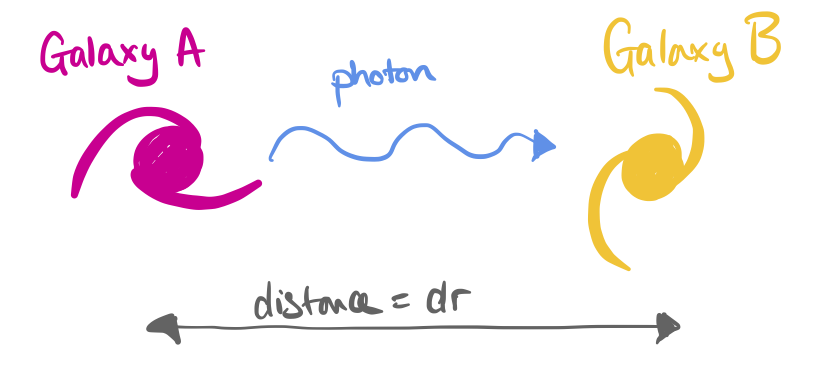
\includegraphics[width=1\linewidth]{Images/redshift-galaxies} \caption{A photon travelling between two galaxies}\label{fig:redshift-galaxies}
\end{figure}

Consider a photon travelling between two points in space, as shown in
Figure \ref{fig:redshift-galaxies}. The relative velocities of the
galaxies in
Fig. \ref{fig:redshift-galaxies} is given by

\begin{equation}
dv = H dr = \dfrac{\dot{a}}{a} dr
\label{eq:red-1}
\end{equation}

We can use the Doppler law to
find the change of the photon's wavelength, \(d\lambda\), while it's
travelling between the two positions

\begin{equation}
\dfrac{d\lambda}{\lambda} = \dfrac{dv}{c}
\label{eq:red-2}
\end{equation}

The travel time of the
photon is \(dt = dr/c\), which we can combine with
Equations \eqref{eq:red-1} and \eqref{eq:red-2}
to find

\begin{equation}
\dfrac{d\lambda}{\lambda} = \dfrac{\dot{a}}{a} \dfrac{dr}{c} = \dfrac{\dot{a}}{a} dt
\label{eq:lambda-a}
\end{equation}

Integrating Equation \eqref{eq:lambda-a} shows that
\(\ln \lambda = \ln a + \text{constant}\), i.e.
\begin{equation}
\lambda \propto a
\label{eq:lambda-a-2}
\end{equation}

The energy of a photon is proportional to its wavelength, so
\begin{equation}
E = \dfrac{h c}{\lambda} \propto \dfrac{1}{a}
\label{eq:lambda-a-3}
\end{equation}
This reduction in
energy by an additional factor of \(a\) accounts for the slowed expansion
in a radiation dominated Universe.

\hypertarget{sec:mixtures}{%
\section{Mixing matter and radiation}\label{sec:mixtures}}

In Sections \ref{sec:matter-eos} and
\ref{sec:radiation-eos} we considered the cases where the
Universe was composed of either only matter or only radiation. This is
not particularly realistic; the Universe contains a mixture of these two
components.

We found that the energy densities of matter and radiation are related
to the scale factor by different amounts, with the radiation energy
density decreasing more quickly as \(a\) increases:

\begin{equation}
\begin{array}{lr}
    \rho_{\text{mat}} \propto \dfrac{1}{a^3} & \qquad
    \rho_{\text{rad}} \propto \dfrac{1}{a^4}
\end{array}
\label{eq:rad-mat-1}
\end{equation}
Even though the Universe is a mixture of matter and
radiation, it still obeys the Friedman equation
(Eqn. \eqref{eq:friedman}) in the same way, with the individual
densities combined into a single value of \(\rho\):
\begin{equation}
\rho = \rho_{\text{mat}} + \rho_{\text{rad}}
\label{eq:rho-mat-rad}
\end{equation}
We could solve the
Friedman equation in full, but in practice only the dominant density term significantly affects the evolution of the scale factor at any
given time.

At early times, the radiation energy density will dominate over the
matter energy density, meaning that \(a\) will evolve as in the radiation
case:
\begin{equation}
a(t) \propto t^{1/2}
\label{eq:a-t}
\end{equation}
Combining this with our individual
equations for \(\rho(t)\) we find
\begin{equation}
\rho_{\text{rad}} \propto \dfrac{1}{t^2}
\label{eq:rho-rad-t}
\end{equation}
for the radiation dominated case, and
\begin{equation}
     \rho_{\text{mat}} \propto \dfrac{1}{a^3} \propto \dfrac{1}{t^{3/2}}
\label{eq:rho-mat-t}
\end{equation}
for the matter dominated case.

\begin{figure}
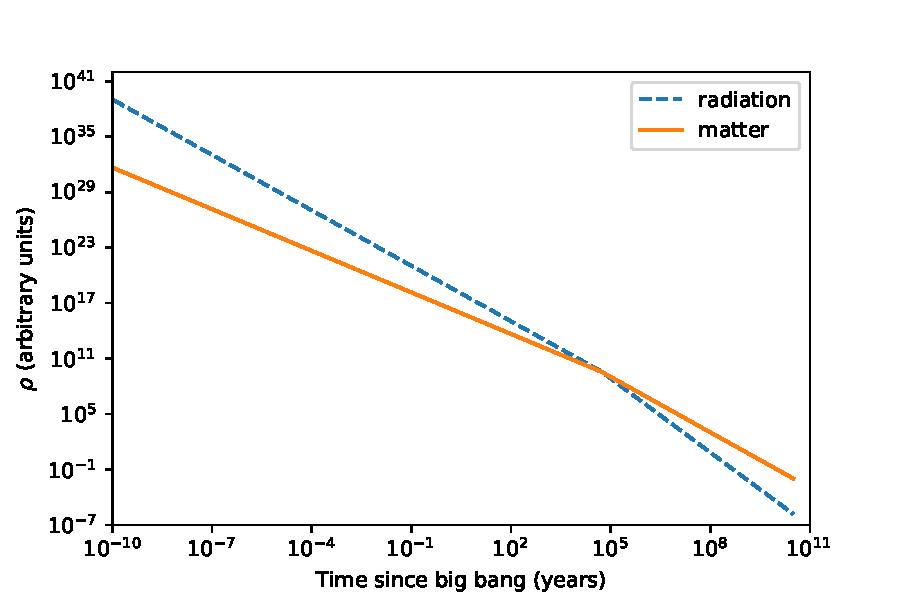
\includegraphics[width=1\linewidth]{Images/density_plot} \caption{Evolution of the matter (orange solid line) and radiation (blue dashed line) density components as a function of time in a mixed composition Universe. Radiation dominates for early times, but as $t$ (hence $a$) increases, matter becomes the dominant component.}\label{fig:density-fig}
\end{figure}

Initially, radiation will dominate. However, as \(t\) increases, the
energy density contribution from matter will dominate over radiation, as
shown in
Figure \ref{fig:density-fig}. However, when the matter density
dominates, \(a\) will evolve as in the matter case:
\begin{equation}
\begin{array}{lcr}
    a(t) \propto t^{2/3} & \qquad
    \rho_{\text{mat}} \propto \dfrac{1}{t^2} & \qquad
    \rho_{\text{rad}} \propto \dfrac{1}{a^4} \propto \dfrac{1}{t^{8/3}}
\end{array}
\label{eq:a-rho-comb}
\end{equation}

\hypertarget{sec:dark_energy_1}{%
\section{Cosmological Constant}\label{sec:dark_energy_1}}

The final case that we haven't considered is the contribution from the
cosmological constant, \(\Lambda\) and its density \(\rho_{\Lambda}\). We
know from observations that the Universe is now in the \(\Lambda\) (Dark
Energy) dominated era, but what does that mean for its evolution?

The fluid equation for \(\Lambda\) is
\begin{equation}
\dot{\rho_{\Lambda}} + 3\frac{\dot{a}}{a} \left(\rho_{\Lambda} + \dfrac{P_{\Lambda}}{c^2}\right) = 0
\label{eq:rho-lambda-1}
\end{equation}
We know that \(\rho_{\Lambda}\) is constant over time, which leads to
\begin{equation}
P_\Lambda = -\rho_{\Lambda}c^2
\label{eq:rho-lambda-2}
\end{equation}
This means that \(\Lambda\) has a
\textbf{negative effective pressure}. As Universe expands, work is done on
the \(\Lambda\) fluid, allowing its density to stay constant even as the
Universe increases in volume. We'll come back to the ridiculousness of
\(\Lambda\) later in the course.

\hypertarget{sec:composition_ex}{%
\section{Exercises}\label{sec:composition_ex}}

\begin{enumerate}
\def\labelenumi{\arabic{enumi}.}
\item
  So far we've looked at the cases for matter, where \(P = 0\), and
  radiation, where \(P = \rho c^2 / 3\). Consider a generic equation of
  state where \(P = (\gamma - 1) \rho c^2\), where \(0 < \gamma < 2\).
  Find equations for \(\rho(a)\), \(a(t)\) and \(\rho(t)\) for this equation
  of state. Assume a flat Universe, i.e. \(k=0\).
\item
  Recall the Friedman equation:
  \[\left(\dfrac{\dot{a}}{a}\right)^2 = \dfrac{8\pi G}{3}\rho - \dfrac{k}{a^2}\]
  Considering the equations you derived in part 1, what value of
  \(\gamma\) is required so that \(\rho\) has the same time dependence as
  the curvature term, \(k/a^2\)?
\item
  Assuming \(k<0\), find the solution \(a(t)\) to the Friedman equation
  for a fluid with the value of \(\gamma\) you derived in Section \ref{sec:geometry-ex}.
\end{enumerate}

\bibliography{book.bib,packages.bib}


\end{document}
